\section{Conclusion}
This project evaluated the knowledge capabilities of three advanced AI models—ChatGPT, Gemini, and Meta AI—by 
analyzing their answers to questions generated from seminar transcriptions. The results revealed that Gemini performed 
the best, achieving an accuracy of 96.75\%, followed by ChatGPT at 87.5\%, and Meta AI at 85\%. 
These findings highlight the strong baseline knowledge of all three AIs, with Gemini demonstrating exceptional accuracy.
\begin{figure}[H]
    \centering
    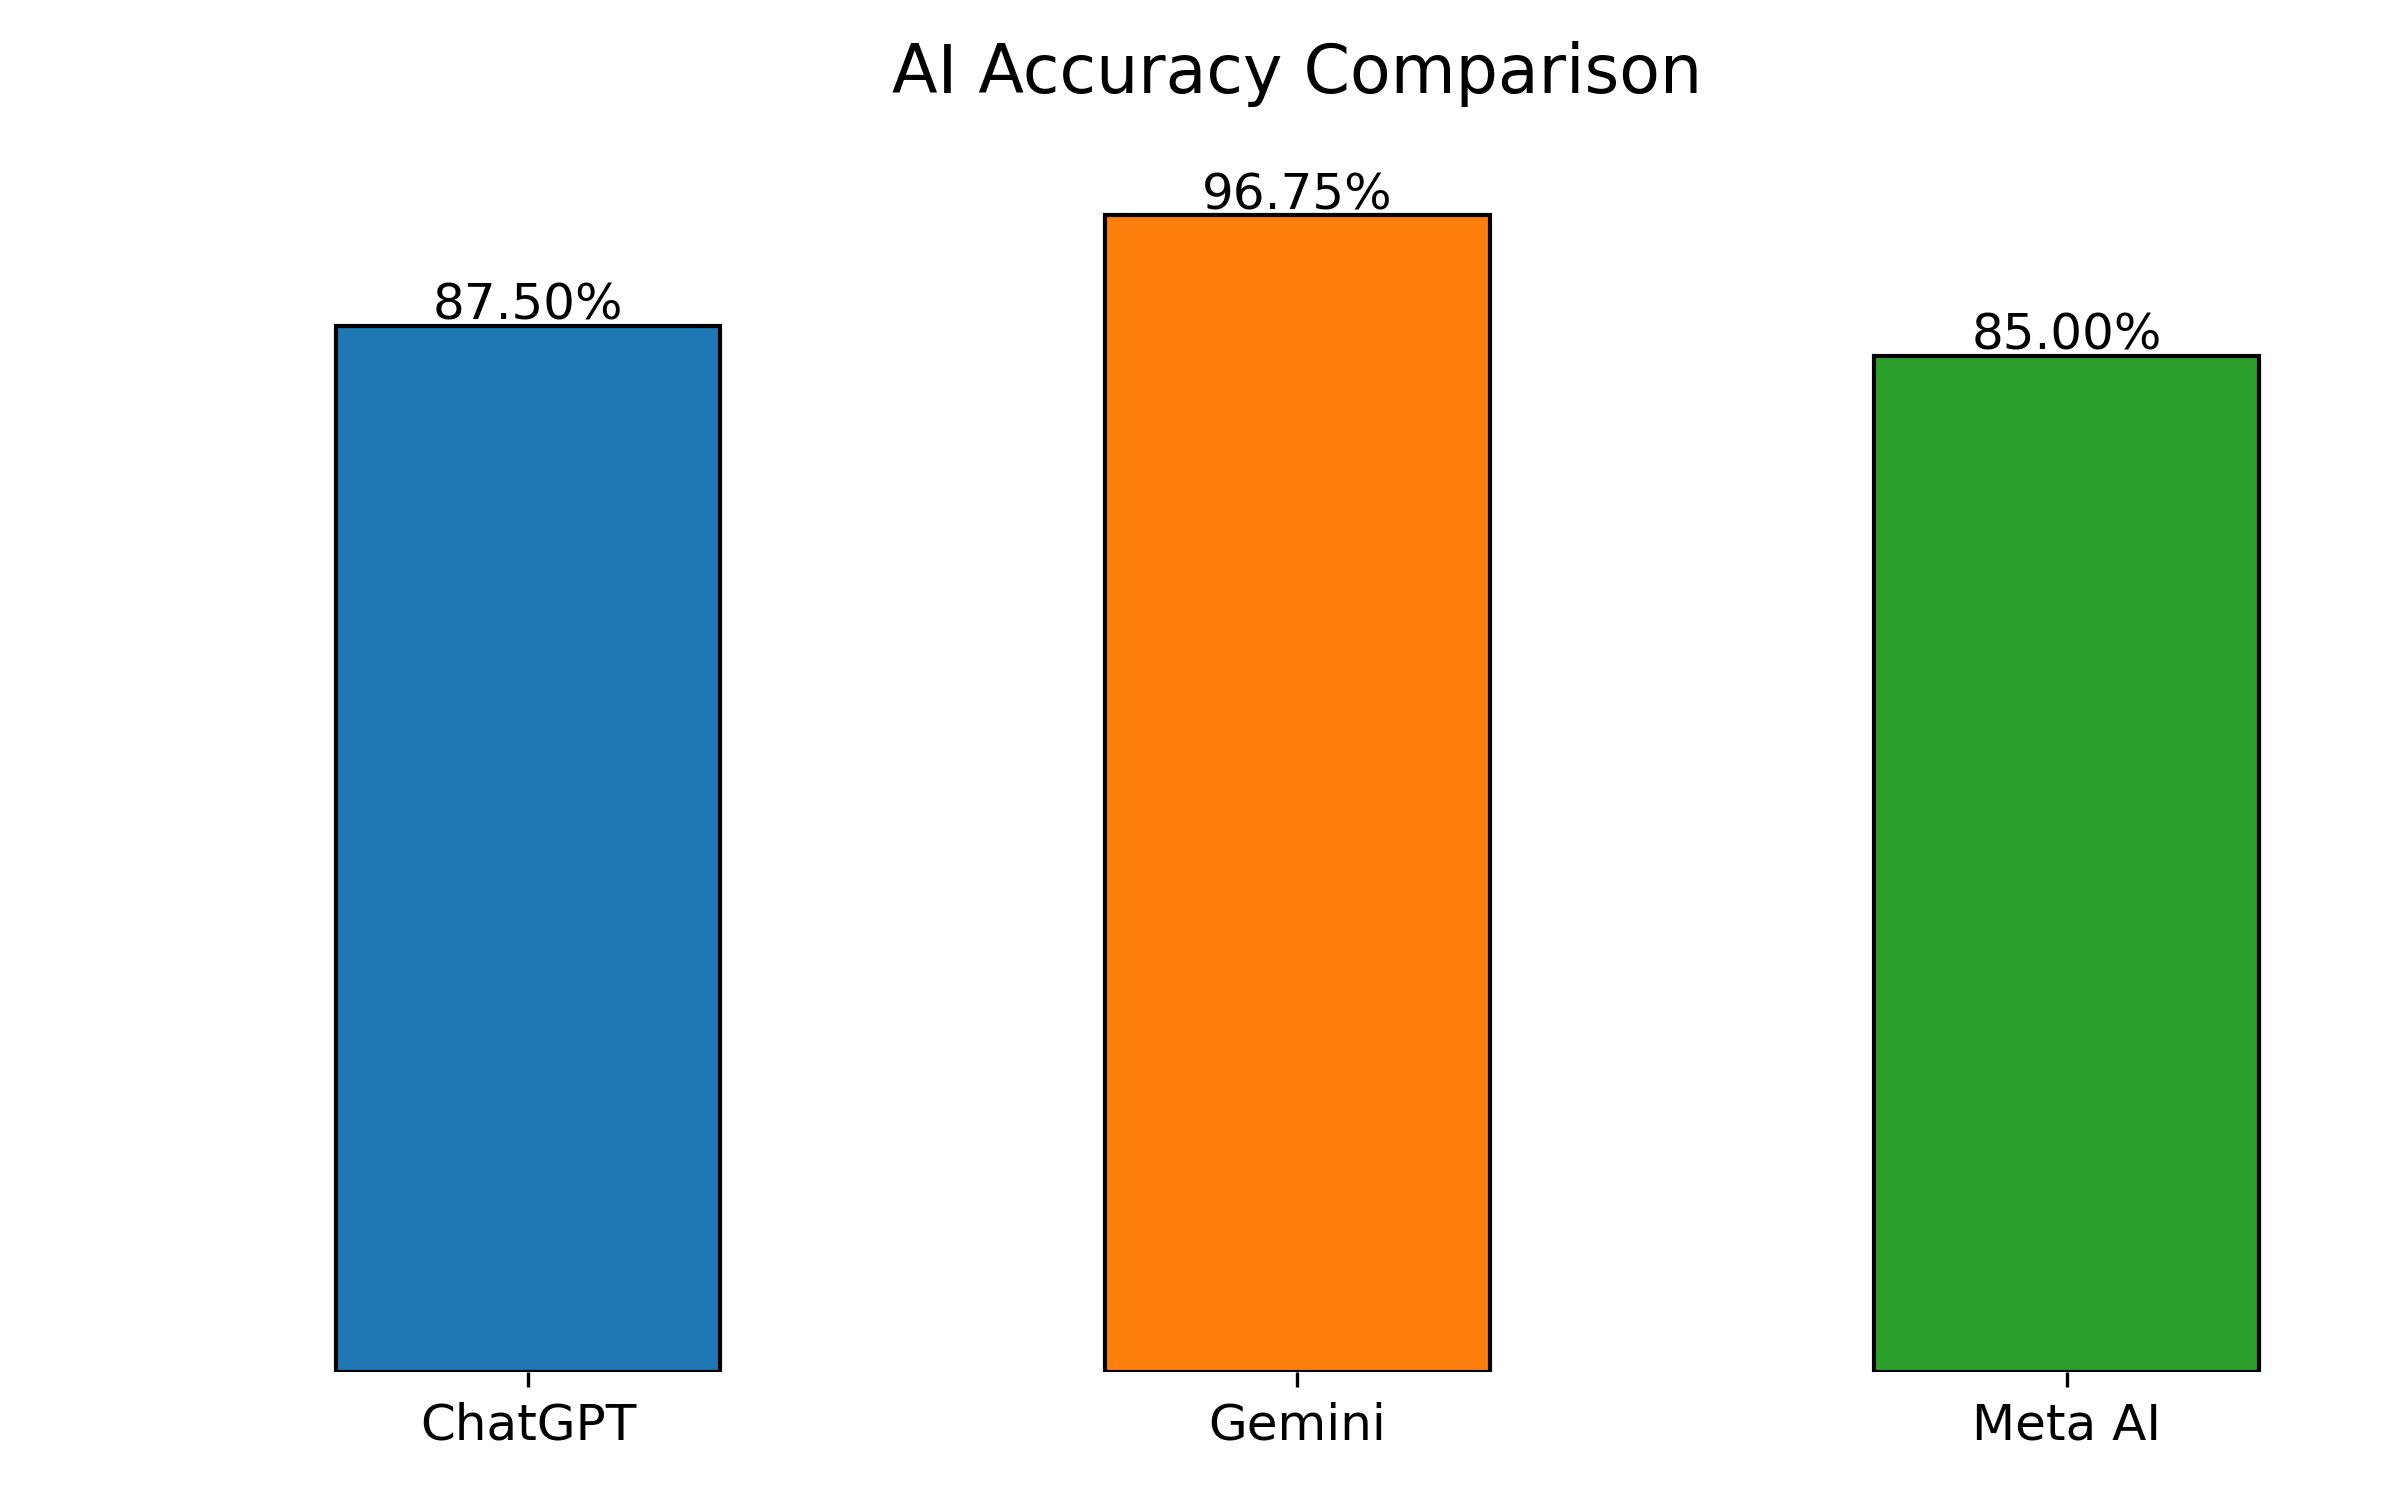
\includegraphics[scale=0.75]{Imagens/graph.jpg}
\end{figure}
A notable challenge in the evaluation process was the use of NotebookLM. While it offered a structured way to assess responses,
its evaluation criteria were inconsistent, often changing between questions. For example, NotebookLM frequently marked
answers as partially correct if specific details mentioned in the seminars were omitted, even when the broader context 
was accurate. Manual analysis showed that most of these flagged answers were actually correct, indicating that the 
evaluation process was overly strict and sometimes misleading.

The inconsistencies in NotebookLM’s evaluation   underscore the need for more stable and reliable assessment tools
in similar projects. Despite these limitations, the results affirm that all three AI models performed impressively,
showcasing their ability to engage with complex topics using only their default knowledge.
